%%=============================================================================
%% Conclusie
%%=============================================================================

\chapter{Conclusie}%
\label{ch:conclusie}

% TODO: Trek een duidelijke conclusie, in de vorm van een antwoord op de
% onderzoeksvra(a)g(en). Wat was jouw bijdrage aan het onderzoeksdomein en
% hoe biedt dit meerwaarde aan het vakgebied/doelgroep? 
% Reflecteer kritisch over het resultaat. In Engelse teksten wordt deze sectie
% ``Discussion'' genoemd. Had je deze uitkomst verwacht? Zijn er zaken die nog
% niet duidelijk zijn?
% Heeft het onderzoek geleid tot nieuwe vragen die uitnodigen tot verder 
%onderzoek?
\section{CPU verbruik}
In de volgende figuren wordt duidelijk dat Environment voordelen biedt op het gebied van CPU-verbruik. Deze conclusie is echter niet volledig vergelijkbaar met andere property wrappers, omdat Environment een specifieke functie vervult. We kunnen daarom concluderen dat Binding het minste CPU-verbruik vereist om objecten door te geven aan een SwiftUI-view. Daarnaast kunnen we uit de volgende tabellen afleiden dat de nieuwere observable macro zwaarder is voor de CPU dan alle andere annotaties.

\subsubsection{binding}
Uit de tabel blijkt dat wanneer we een binding gebruiken om een groot object door te geven aan een view, en we maken een aanpassing in die view, dit ongeveer 14,08 mega cycli van de CPU vereist.
\begin{figure}[htbp]
    \centering
    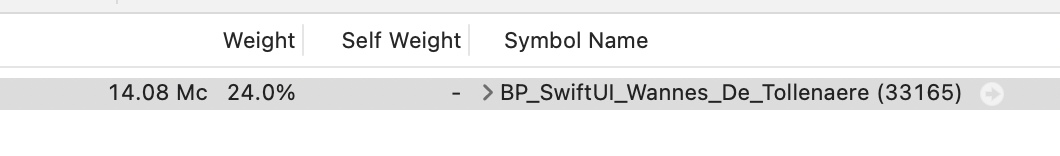
\includegraphics[width=1\textwidth]{BP_CpuUsageBinding} 
    \caption{CPU gebruik van binding}
    \label{fig:cpuBinding}
\end{figure}

\subsubsection{environment}
Uit de tabel blijkt dat het gebruik van Environment om een groot object door te geven aan een view, en het vervolgens aanpassen van dat object, ongeveer 250,08 kilocycli van de CPU vereist.
\begin{figure}[htbp]
    \centering
    
\includegraphics[width=1\textwidth]{BP_CpuUsageEnvironment} 
    \caption{CPU gebruik van environment}
    \label{fig:cpuEnvironment}
\end{figure}

\subsubsection{environmentObject}
Uit de tabel blijkt dat het gebruik van een environmentObject om een groot object door te geven aan een view, en het vervolgens aanpassen van dat object, ongeveer 17,13 mega cycli van de CPU vereist.
\begin{figure}[htbp]
    \centering
    
\includegraphics[width=1\textwidth]{BP_CpuUsageEnvironmentObject} 
    \caption{CPU gebruik van environmentObject}
    \label{fig:cpuEnvironmentObject}
\end{figure}

\subsubsection{observable}
Uit de tabel blijkt dat wanneer we een Observable gebruiken om een groot object door te geven aan een view, en we vervolgens een aanpassing aan dat object in die view maken, dit ongeveer 19,45 mega cycli van de CPU vereist.
\begin{figure}[htbp]
    \centering
    
\includegraphics[width=1\textwidth]{BP_CpuUsageObservable} 
    \caption{CPU gebruik van een Observable}
    \label{fig:cpuObservable}
\end{figure}\

\subsubsection{observableObject}
Uit de tabel blijkt dat wanneer we een observableObject gebruiken om een groot object door te geven aan een view, en we vervolgens een aanpassing aan dat object in die view maken, dit ongeveer 17,82 mega cycli van de CPU vereist.
\begin{figure}[htbp]
    \centering
    
\includegraphics[width=1\textwidth]{BP_CpuUsageObservedObject} 
    \caption{CPU gebruik van observableObject}
    \label{fig:cpuObservedObject}
\end{figure}

\subsubsection{observableObject}
Uit de tabel blijkt dat het simpelweg doorgeven van een groot object aan een view zonder speciale annotaties, en zonder er vervolgens aanpassingen op te maken, gemiddeld 2,00 mega cycli van de CPU verbruikt.
\begin{figure}[htbp]
    \centering
    
\includegraphics[width=1\textwidth]{BP_CpuUsageWithoutPropertyWrapper} 
    \caption{CPU gebruik van een view zonder property wrappers}
    \label{fig:cpuWithoutPropertyWrapper}
\end{figure}


\newpage
\section{Property updates}

Na 101 keer een aanpassing door te voeren op een groot object en dat aan de overdrachtsmethode te koppelen, zien we dat Binding, ObservedObject en EnvironmentObject de property 202 keer hebben bijgewerkt, terwijl Observable en Environment de property slechts 101 keer hebben bijgewerkt. Dit verschil in updatefrequentie heeft invloed op de nauwkeurigheid en consistentie van de state van de applicatie, wat belangrijk is voor een responsieve gebruikerservaring. Echter, te vaak updaten kan leiden tot een hogere CPU-belasting en minder efficiënte prestaties.

Binding, ObservedObject en EnvironmentObject passen de property bij elke wijziging tweemaal aan, wat zorgt voor een snellere en consistenter bijgewerkte state. Deze methoden zijn geschikt voor applicaties waarbij real-time gegevensuitwisseling en een directe reactie op veranderingen essentieel zijn, zoals een chatapplicatie of een live-dashboard.

Daarentegen voeren Observable en Environment slechts één update per aanpassing uit, wat kan resulteren in minder efficiënte of langzamere reacties op veranderingen. Deze methoden kunnen beter geschikt zijn voor applicaties waar updates minder frequent zijn of waar de responsietijd minder kritisch is, zoals een notitie-app of een takenbeheer-app.

Het is belangrijk om de juiste overdrachtsmethode te kiezen op basis van de behoeften van de applicatie en de frequentie van wijzigingen om een goede balans te vinden tussen het bijwerken van properties en de efficiëntie van het systeem.

\begin{figure}[htbp]
    \centering
    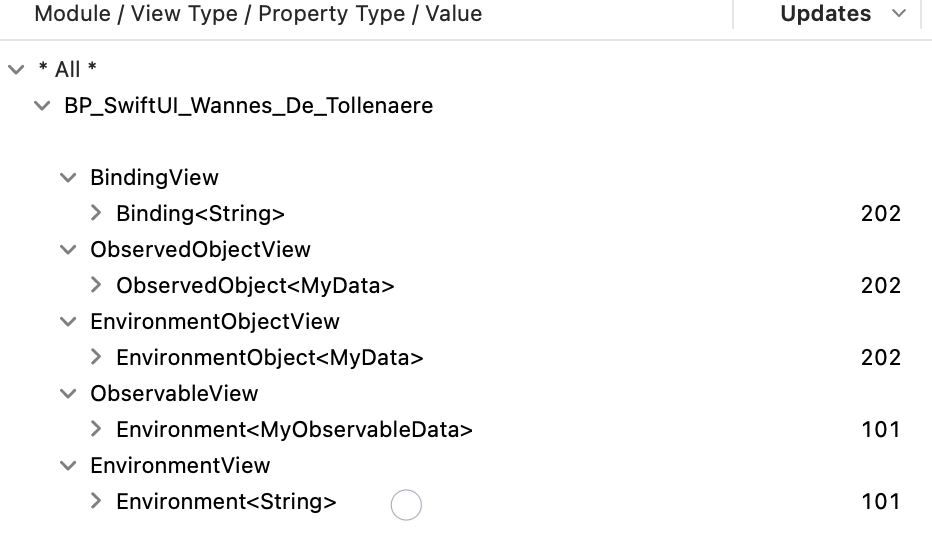
\includegraphics[width=1\textwidth]{BP_ViewPropertyUpdates} 
    \caption{Aantal keren dat de property's geupdate zijn bij het 101 keer opnieuw toewijzen}
    \label{fig:propertyUpdates}
\end{figure}

\newpage
\section{View refresh time}
Op basis van de gemiddelde view refresh times die zijn gemeten voor de verschillende manieren van data-binding in SwiftUI, kunnen de volgende conclusies worden getrokken:

\subsection{Observable en EnvironmentObject}
Deze methoden laten de snelste refresh times zien, met respectievelijk 2.52 en 2.69 microseconden. Dit suggereert dat deze benaderingen efficiënter zijn in het updaten van de UI wanneer de onderliggende data verandert. Dit kan worden toegeschreven aan de geoptimaliseerde manier waarop Observable en EnvironmentObject werken in SwiftUI, waarbij Observable expliciete meldingen van datawijzigingen mogelijk maakt, en EnvironmentObject een efficiënte, globale benadering biedt.

\subsection{Environment}
De gemiddelde refresh time voor Environment (2.87 microseconden) ligt dicht bij die van Observable en EnvironmentObject. Dit duidt op een vergelijkbare efficiëntie, maar mogelijk iets minder optimaal vanwege de bredere reikwijdte van het gebruik van Environment in SwiftUI-applicaties.

\subsection{Binding}
Met een gemiddelde refresh time van 3.23 microseconden is binding iets minder efficiënt dan Observable en EnvironmentObject. Dit kan worden verklaard door de manier waarop binding werkt, wat meer overhead kan introduceren in vergelijking met de directe datawijzigingen van Observable en EnvironmentObject.

\subsection{ObservedObject}
Deze methode laat de traagste refresh time zien (4.22 microseconden) in vergelijking met de andere benaderingen. Dit kan duiden op een hoger overheadniveau of minder optimalisaties in de manier waarop ObservedObject wordt gebruikt voor het volgen en updaten van UI-componenten.

\paragraph{conclusie}
Over het algemeen lijken Observable en EnvironmentObject de meest efficiënte benaderingen voor het snel updaten van de UI in SwiftUI-applicaties. Binding en ObservedObject zijn minder efficiënt en kunnen mogelijk extra overhead toevoegen. Deze bevindingen kunnen ontwikkelaars helpen bij het kiezen van de meest geschikte data-binding benadering voor hun SwiftUI-applicaties.

\begin{figure}[htbp]
    \centering
    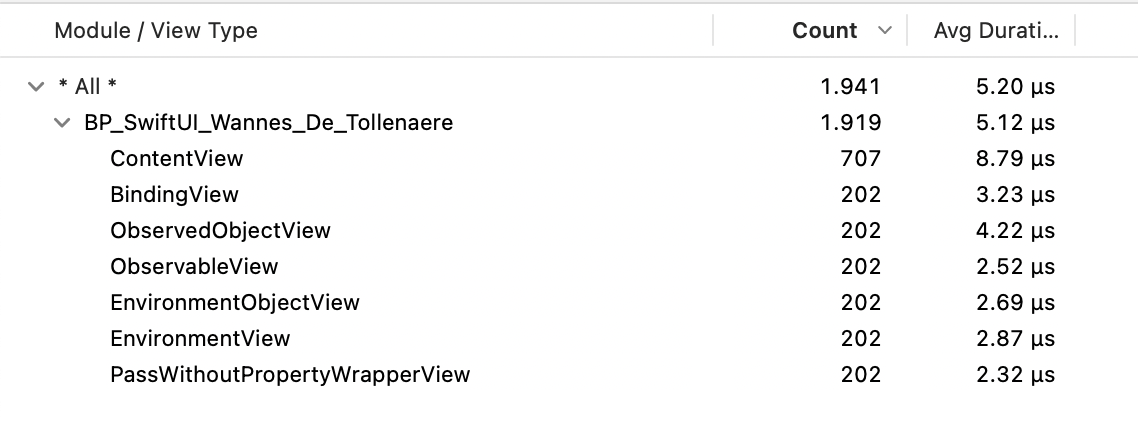
\includegraphics[width=1\textwidth]{BP_ViewRefreshCountAvgDuration} 
    \caption{Gemiddelde duratie voor de view om in te laden per property type}
    \label{fig:propertyRefreshDuration}
\end{figure}

\newpage
\section{Nieuwe Observable macro}
Op basis van de besproken gegevens met betrekking tot Observable in vergelijking met de andere methoden voor data-binding in SwiftUI, kunnen de volgende conclusies worden getrokken:
\subsection{refresh times}
Observable biedt een van de snelste refresh times (2.52 microseconden) onder de onderzochte methoden. Dit betekent dat het updaten van de UI met Observable efficiënt en snel verloopt, wat resulteert in een responsieve gebruikerservaring.
\subsection{CPU-verbruik}
Observable heeft echter een hoger CPU-verbruik (19.45 megacycli) in vergelijking met andere methoden, zoals Binding (14.08 megacycli). Dit kan een nadeel zijn als je probeert CPU-gebruik te minimaliseren.
\subsection{Property Updates}
Observable voert slechts één update per aanpassing uit, wat leidt tot een lagere updatefrequentie vergeleken met Binding, ObservedObject en EnvironmentObject, die tweemaal updaten per aanpassing. Dit kan in sommige gevallen resulteren in langzamere reacties op veranderingen.
\subsection{Gebruikssituaties}
Door de efficiënte refresh times en lagere updatefrequentie kan Observable een goede keuze zijn voor applicaties waar snelheid belangrijk is en waar updates minder frequent zijn. In situaties waarin nauwkeurige en consistente state-updates van cruciaal belang zijn, kunnen echter andere methoden, zoals Binding, ObservedObject, of EnvironmentObject, geschikter zijn.
 
\newpage
\section{Aanbevelingen}
Door rekening te houden met deze conclusies en aanbevelingen, kunt u de juiste keuzes maken bij het ontwerpen van SwiftUI-applicaties, en zo een goede balans vinden tussen efficiëntie, snelheid en consistentie.
\subsection{Kies de juiste methode voor specifieke behoeften}
Gebruik Observable en EnvironmentObject wanneer snelheid en efficiëntie in het updaten van de UI prioriteit hebben.
Environment biedt een gebalanceerde aanpak voor het delen van data over verschillende componenten heen.
\subsection{overhead}
Binding en ObservedObject kunnen meer overhead en trager CPU-verbruik veroorzaken. Gebruik ze met voorzichtigheid, vooral als prestaties belangrijk zijn.
\subsection{frequentie van updates}
Kies een benadering die past bij de frequentie van updates in uw applicatie. Meer updates zorgen voor een snellere state, maar kunnen ook de CPU-belasting verhogen.




